Um die Laufzeitanalyse durchzuführen, wurde unter C++ die Bibliothek \code{std::chrono} verwendet. Unter C kam die etwas ungenauere Funktion \code{clock()} zum Einsatz. Bei dem Testsystem handelt es sich um eine x64 AMD-Plattform der Zen 2 Generation mit 4,00 GHz und 3600 MHz DDR4-Speicher. Die Ergebnisse sind somit nicht mit anderen Systemen zu vergleichen, da diese stark plattformabhängig sind. Die Zeitmessungen wurden nach dem Einlesen der Chipsequenz gestartet und unmittelbar nach der Decodierung beendet. Somit beschreibt die Zeitspanne ausschließlich die Decodierung selbst und die Schritte, welche dafür nötig sind, wie zum Beispiel die Generierung der Goldsequenzen.

Nachfolgend ist die Betrachtung für C++, die unoptimierte, sowie die optimierte C-Implementierung aufgeführt mit jeweils dem Debug- und Release-Build. 
Im Debug-Build ist die Compilerseite Optimierung ausgeschaltet und Debuginformationen sind zugelassen. Der Release-Build speichert keinerlei Debuginformationen, verwendet die höchste verfügbare Optimierungsstufe mit Priorisierung von Geschwindigkeit (O3 bei GCC, O2 bei MSVC) und lässt Funktionsinlining zu.

\subsection{C++}
\begin{figure}[H]
	\centering
	\begin{subfigure}{.5\textwidth}
		\centering
		\includegraphics[width=\linewidth]{\imagePath/C++/debug.png}
		\caption{Debug-Build.}
		\label{fig:cpp_debug}
	\end{subfigure}%
	\begin{subfigure}{.5\textwidth}
		\centering
		\includegraphics[width=\linewidth]{\imagePath/C++/release.png}
		\caption{Release-Build.}
		\label{fig:cpp_release}
	\end{subfigure}
	\caption{Die Konsolenausgaben der jeweiligen Builds der C++-Implementierung. Links: der Debug-Build. Rechts: der Release-Build. Die Geschwindigkeitszunahme bei Anschalten der Compileroptimierungen ist enorm. Die Laufzeit von etwa 8 Sekunden im Debug sanken auf etwa 72 Millisekunden im Release. Das ergibt eine Geschwindigkeitssteigerung um den Faktor 111.}
	\label{fig:cpp}
\end{figure}

\subsection{C unoptimiert}
\begin{figure}[H]
	\centering
	\begin{subfigure}{.5\textwidth}
		\centering
		\includegraphics[width=\linewidth]{\imagePath/C_unoptimized/debug.png}
		\caption{Debug-Build.}
		\label{fig:c_unoptimized_debug}
	\end{subfigure}%
	\begin{subfigure}{.5\textwidth}
		\centering
		\includegraphics[width=\linewidth]{\imagePath/C_unoptimized/release.png}
		\caption{Release-Build.}
		\label{fig:c_unoptimized_release}
	\end{subfigure}
	\caption{Die Konsolenausgaben jeweiliger Builds der unoptimierten C-Implementierung. Links: der Debug-Build. Rechts: der Release-Build. Der Geschwindigkeitszuwachs im Release ist mit Halbierung der Laufzeit  vergleichsweise zur C++-Implementierung nicht ansatzweise so groß.}
	\label{fig:c_unoptimized}
\end{figure}

\subsection{C optimiert}
\begin{figure}[H]
	\centering
	\begin{subfigure}{.5\textwidth}
		\centering
		\includegraphics[width=\linewidth]{\imagePath/C_optimized/debug.png}
		\caption{Debug-Build.}
		\label{fig:c_optimized_debug}
	\end{subfigure}%
	\begin{subfigure}{.5\textwidth}
		\centering
		\includegraphics[width=\linewidth]{\imagePath/C_optimized/release.png}
		\caption{Release-Build.}
		\label{fig:c_optimized_release}
	\end{subfigure}
	\caption{Die jeweiligen Build-Ausgaben der optimierten C-Implementierung. Links: der Debug-Build. Rechts: der Release-Build. Der Geschwindigkeitszuwachs von Debug zu Release ist auch hier nicht so groß wie in C++, aber dennoch größer als in der unoptimierten C Implementierung. Der Release ist etwa 5 Mal schneller als der Debug-Build.}
	\label{fig:c_optimized}
\end{figure}

Um die Laufzeit des C-Programms zu verringern, sind zunächst triviale Optimierungen der Sprache vorgenommen worden. Darunter fallen:
\begin{enumerate}
	\item Konstante Werte wurden durch Präprozessordefinitionen ersetzt.
	\item Die Funktion\code{\_correlate()} in dem Modul \code{Decoder} wurde in die Funktion \\ \code{CDMA\_decode()} eingefügt.
	\item Zählervariabeln erhielten das Schlüsselwort \code{register}.
	\item Es wurden Prä- statt Postinkrements verwendet.
	\item Bei Iteration über Pointer wurde auf Indexzugriff verzichtet und stattdessen ein Zeiger inkrementiert.
\end{enumerate}
Das alles sind Optimierungen, die der Compiler ohnehin vorgenommen hätte. Sie verringern allerdings bereits die Zeit im Debug-Build um einige Millisekunden. 
Weitere programmspezifische Verbesserungen erzielten die größten Zeiteinsparungen und verringerten die Ausführungszeit nochmals um wenige 10 Millisekunden:
\begin{enumerate}
	\item Ein "Early-Exit" bricht die Korrelation ab, wenn bereits alle gesendeten Bits gefunden wurden. Diese Abfrage erzielt vor allem bei Bitsendungen von niedrig indexierten Satelliten große Verbesserung. Im schlimmsten Fall, das heißt der 24. Satellit sendet, läuft das Programm minimal langsamer. 
	\item Da die Goldsequenzen immer gleich sind, müssen sie nicht vor jeder Decodierung neu berechnet werden. Es reicht, diese einmal zu generieren und dann wiederzuverwenden. Ein zweidimensionales Stack-Array speichert die Goldfolgen als lokale Variable in der decode-Funktion, auf welche dann nur noch lesend zugegriffen wird.
	\item Der Modulo-Operator, welcher zur Begrenzung des Index zum Zugriff auf die Goldsequenz dient, befindet sich in der inneren Schleife, wird oft ausgeführt und ist damit sehr teuer. Um darauf zu verzichten, wurde zunächst eine Methode der Bitmanipulation eingesetzt \footnote{https://graphics.stanford.edu/~seander/bithacks.html\#ModulusDivisionParallel}, welche aber durch die Duplizierung der Goldsequenzen ersetzt wurde. Somit konnte auf Kosten der Speicherlast auf den Modulo-Operator komplett verzichtet und die Laufzeit um einiges verbessert werden.
	\item Die letzte Optimierung wurde ebenfalls in der inneren Schleife angewandt, um auf den ternären Operator sowie auf den unären Negationsoperator bei der Akkumulation zu verzichten. Dabei sind die Goldfolgen nun nicht länger als eine Menge aus $ 1 $ und $ 0 $ repräsentiert. Anstelle der $ 0 $ wird $ -1 $ gespeichert, welche mit dem entsprechenden Eintrag in der Chipsequenz verrechnet werden kann, um das gewünschte Ergebnis zu erzielen.
\end{enumerate}